\begin{figure}[th!]
\caption{Week 8: Question 1 results}
\centering
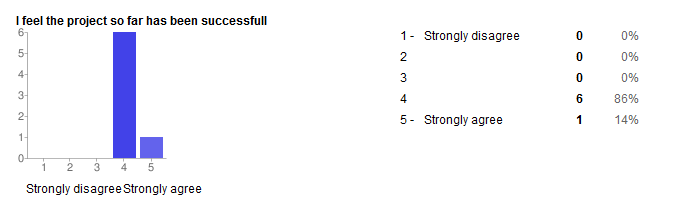
\includegraphics[width=0.9\textwidth]{evaluation/week_8_images/project_successfull}
\label{fig:W8Q1}
\end{figure}

In Figure~\ref{fig:W8Q1} we can see that the group agrees that the project is successfull, meaning that we feel the project process is going as scheduled, and that the overall motivation is high. 

\begin{figure}[th!]
\caption{Week 8: Question 2 results}
\centering
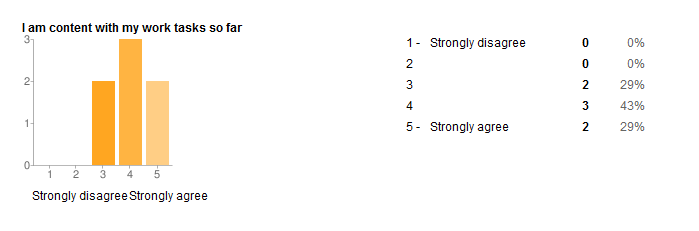
\includegraphics[width=0.9\textwidth]{evaluation/week_8_images/work_tasks}
\label{fig:W8Q2}
\end{figure}

In Figure~\ref{fig:W8Q2} we see that most of the group members are also happy with their work tasks so far. We have had pretty static roles with a documentation team and a programming team so far, and these results tell us that this model has worked for our group. However, for the last 3 weeks, all team membres will be on the documentation team.

\begin{figure}[th!]
\caption{Week 8: Question 3 results}
\centering
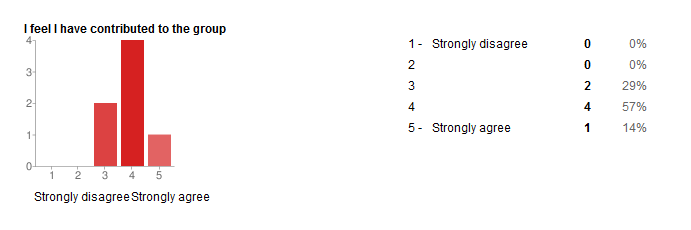
\includegraphics[width=0.9\textwidth]{evaluation/week_8_images/contributed_group}
\label{fig:W8Q3}
\end{figure}

Figure~\ref{fig:W8Q3} shows that most group members feel that they have contributed to the group. At our internal review meeting of the results, it was also discussed that the other team members felt that all members of the group contributed, which helped motivate themselves. 

\begin{figure}[th!]
\caption{Week 8: Question 4 results}
\centering
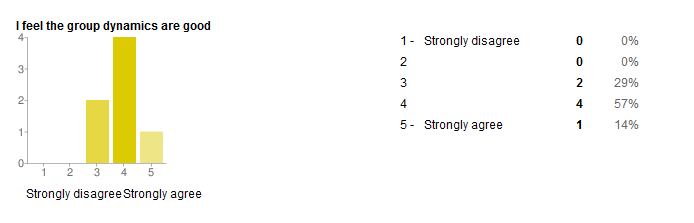
\includegraphics[width=0.9\textwidth]{evaluation/week_8_images/group_dynamics}
\label{fig:W8Q4}
\end{figure}

\begin{figure}[th!]
\caption{Week 8: Question 5 results}
\centering
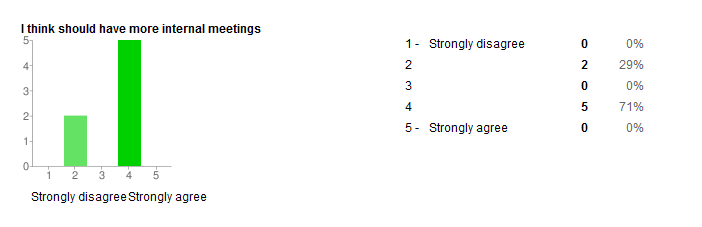
\includegraphics[width=0.9\textwidth]{evaluation/week_8_images/internal_meetings}
\label{fig:W8Q5}
\end{figure}
 The most important finding of our midproject review was by far the results from Figure~\ref{fig:W8Q5}. The concensus of the group was that we had too few meetings, which halted communication between the team members. This meant that motivation dropped, or that one part of the group didn't know what the other part was doing, leading to the results in Figure~\ref{fig:W8Q9}. This also had an impact on motivation and progress for the documentation team. We will from now have weekly meetings each monday with a more fulfilling update form the week before, and plan for the next week.

\begin{figure}[th!]
\caption{Week 8: Question 6 results}
\centering
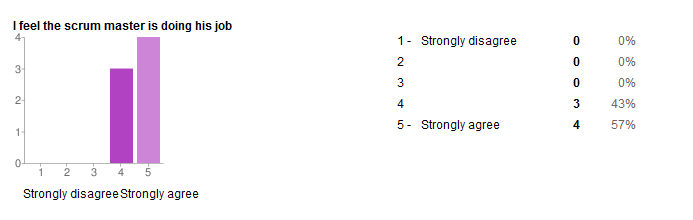
\includegraphics[width=0.9\textwidth]{evaluation/week_8_images/scrum_master}
\label{fig:W8Q6}
\end{figure}

\begin{figure}[th!]
\caption{Week 8: Question 7 results}
\centering
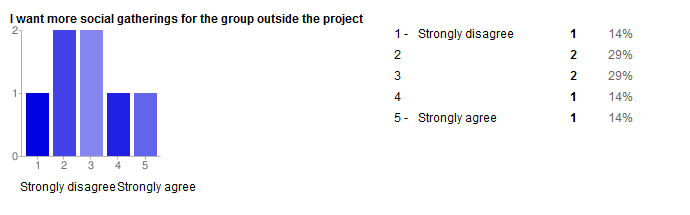
\includegraphics[width=0.9\textwidth]{evaluation/week_8_images/social}
\label{fig:W8Q7}
\end{figure}

\begin{figure}[th!]
\caption{Week 8: Question 8 results}
\centering
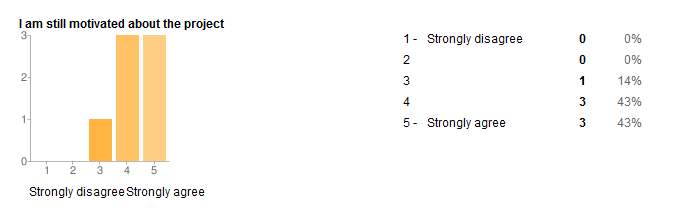
\includegraphics[width=0.9\textwidth]{evaluation/week_8_images/i_motivated}
\label{fig:W8Q8}
\end{figure}

\begin{figure}[th!]
\caption{Week 8: Question 9 results}
\centering
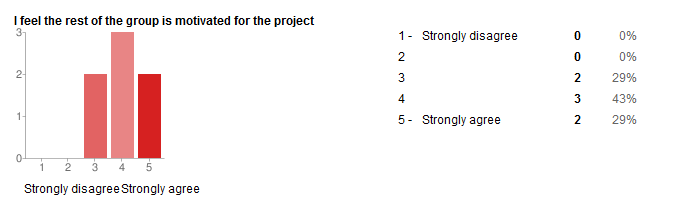
\includegraphics[width=0.9\textwidth]{evaluation/week_8_images/them_motivated}
\label{fig:W8Q9}
\end{figure}

Figure~\ref{fig:W8Q8} and~\ref{fig:W8Q9} shows some interesting results. Most of the group is still motivated about the project, but almost everyone feels that everyone else is less motivated than themselves. While a loss of motivation as the project progresses is to be expected, this was an interesting finding. We came to the conclusion that this was because of the lack of weekly updates between the teams, and sometimes even internally in the teams.

\begin{figure}[th!]
\caption{Week 8: Question 10 results}
\centering
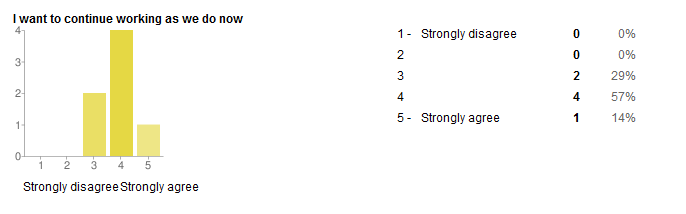
\includegraphics[width=0.9\textwidth]{evaluation/week_8_images/continue_work}
\label{fig:W8Q10}
\end{figure}

Figure~\ref{W8Q10} shows the results of the most important question of the questionnarie. As we can see, the results are pretty spread, but for the most part, the group would like to continue as we do now. After a group discussion, everyone agreed that with the conclusions from this questionnarie, they would be happy with our work the rest of the project. 
